\input my_macros.tex
%\documentclass[10pt]{article}
\documentclass[final]{siamltex}
\usepackage{amssymb,amsbsy,amsmath,amsfonts,amssymb,amscd,exscale,epic,epsfig,graphicx,algorithm,algorithmic, subfigure, fullpage}
\usepackage{tabularx, pifont, subfig, booktabs}
\usepackage{pseudocode}
%\usepackage[pdftex,bookmarks=false]{hyperref}
\renewcommand\tabularxcolumn[1]{>{\small}m{#1}}
\newcolumntype{Y}{>{\small\centering\arraybackslash}X}
\newcolumntype{Z}{>{\small\arraybackslash}X}
\makeatletter
\newcommand{\rmnum}[1]{\romannumeral #1}
\newcommand{\Rmnum}[1]{\small{\expandafter\@slowromancap\romannumeral #1@}}
\makeatother
%\renewcommand{\baselinestretch}{1.5}
\newcommand{\nchoosek}[2]{\left(\begin{array}{c}#1\\#2\end{array}\right)}
\newcommand{\mcaption}[2]{\caption{\small \em #1}\label{#2}}
\newtheorem{remark}{{\it Remark}\rm }

\usepackage{soul}
\usepackage{lineno}
\usepackage[rightbars,color]{changebar}
\setlength\changebarwidth{6pt}


\newcommand{\Lp}{\left(\frac{L}{p}\right)^3}

\begin{document}
\title{A massively parallel algorithm for computing generalized Gauss transforms \thanks{}}
\author{Rahul S. Sampath\and Hari Sundar\and Shravan K. Veerapaneni}
\maketitle

\begin{abstract}

\end{abstract}
%
\begin{keywords} 
Gauss transform, fast algorithms, heat potentials, high-order
accuracy, tensor-product grids
\end{keywords}
%
\begin{AMS}
35K05, 31A10, 65N38, 65Y20
\end{AMS}
%

\section{Introduction} \label{sc:intro}
Gauss transform is one of several discrete spatial transforms of the form 
%
\beq F(x_j) = \sum_{k=1}^N \kernel f_k \quad \text{at} \quad \{ x_j \, | \, j = 1,...,M \} \, , \label{gt} \eeq
\[\text{where} \quad x_j, y_k \in \mathbb{R}^d. \]
%
The kernel $G_\delta$ is a smooth exponentially decaying function in both the physical
and Fourier domains. The parameter $\delta$ controls how rapidly the kernel decays.  
In the Gauss transform case, $\kernel = e^{-\frac{\|x_j - y_k\|^2}{\delta}}$.  We call the
points $x$ as targets and $y$ as sources.  

Discrete sums of the form (\ref{gt}) are encountered in a variety of disciplines including computational physics, machine learning, computational finance and computer graphics. If the kernel decays rapidly, one can simply truncate the sum to a few neighboring sources at each target. However, in many important applications, this is not the case and computing these sums directly takes $\bigO(NM)$ time. 

Starting from the earlier work of Greengard and Strain \cite{fgt}, several sequential algorithms have 
been proposed (e.g.,  \cite{greengard98, duraiswami03, tausch09, fggt}) to reduce the 
cost to an optimal $\bigO(N+M)$. However, to our knowledge, there have been no parallel implementations to date. 

\paragraph{Contributions} The main contributions of this work are given below.
\begin{itemize} 
%
\item We present a first ever parallel implementation of the fast gauss transform for an 
uniform distribution of points. We incorporate the accelerations introduced in \cite{fggt} for tensor product grids. 
Thereby, the complexity constants in our scheme scale linearly with the number of dimensions 
as opposed to exponential growth. 
%
\item We present a novel scheme for the translation of plane wave expansions; this is one
of the steps in the sequential fast gauss transform algorithm. This new scheme reduces the 
computation and storage costs compared to the previous implementations, especially for highly
non-uniform point distributions.
%
\item We extend our schemes to nonuniform distributions. OCTREES.

\item The cost FGT grows for smaller values of $\delta$. In the nonuniform case, 
We present a scheme that scales well in all ranges of the parameters. It is an extension of the tree-splitting scheme proposed in \cite{veerapaneni08} for computing continuous Gauss transforms. 
%
\end{itemize}

The rest of the paper is organized as follows. In Section \ref{sc:fgt}, we give a high-level description of the sequential FGT algorithm for uniform point distributions. We introduce a novel translation scheme in Section \ref{sc:sweep}. This scheme is slightly (nearly twice) more expensive compared to the {\em sweeping algorithm} introduced in \cite{greengard98} but it significantly improves the storage cost for nonuniform distributions. We also discuss its parallel implementation. In Section \ref{sc:nonuniform}, we will present our octree-based sequential and parallel algorithms for nonuniform distributions. Finally, in Section \ref{sc:results}, we will present scalability results of our algorithm using a variety of test cases. 



\section{Pseudocode} \label{sc:pseudocode}
  

\begin{center}
\begin{pseudocode}[doublebox]{PNUFGT}{N, \delta}
\label{alg:pnufgt}
\COMMENT{Computes $y = S x$} \\
\mbox{Send $x$ from $\widehat{L}$ to $\widehat{R}$} \\
\mbox{Compute $i^{(\widehat{L})} = K_{II}^{(\widehat{L})} x$} \\
\mbox{Compute $i^{(\widehat{R})} = K_{II}^{(\widehat{R})} x$} \\
\mbox{Compute $v_{\widehat{L}} = K_{\widehat{L}I} x$} \\
\mbox{Compute $v_{\widehat{R}} = K_{\widehat{R}I} x$} \\
\mbox{Solve $K_{\widehat{L}\widehat{L}} w_{\widehat{L}} = v_{\widehat{L}}$} \\
\mbox{Solve $K_{\widehat{R}\widehat{R}} w_{\widehat{R}} = v_{\widehat{R}}$} \\
\mbox{Compute $z^{(\widehat{L})} = K_{I\widehat{L}} w_{\widehat{L}}$} \\
\mbox{Compute $z^{(\widehat{R})} = K_{I\widehat{R}} w_{\widehat{R}}$} \\
\mbox{Compute $y^{(\widehat{L})} = i^{(\widehat{L})} - z^{(\widehat{L})}$} \\
\mbox{Compute $y^{(\widehat{R})} = i^{(\widehat{R})} - z^{(\widehat{R})}$} \\
\mbox{Send $y^{(\widehat{R})}$ from $\widehat{R}$ to $\widehat{L}$} \\
\mbox{Compute $y = y^{(\widehat{L})} + y^{(\widehat{R})}$} \\
\RETURN{y}
\end{pseudocode}
\end{center}

%\section{The Fast Algorithm} \label{sc:algo}
%\input{algo.tex}

%\section{Results} \label{sc:results}
%\begin{table}[h!]
\small
\begin{center}
\begin{tabular}{|c|c|c|c|c|}
\hline
Operation & Max. Time & Avg. Time & Max. Flops & Avg. Flops\\
\hline
S2W & & & & \\
\hline
W2L & & & & \\
\hline
L2T & & & & \\
\hline
Total & & & & \\
\hline
\end{tabular}
\end{center}
\caption{{\rm {\footnotesize Timings on 37,268 ($32^3$) processors on Jaguar. The point distribution is uniform random, the parameter $\delta = 8 \times 10^{-4}$ and precision $\epsilon = 10^{-6}$}. Each processor has a million points.}}
\label{t:scaling}
\end{table}

\begin{figure}
	\begin{center}
	
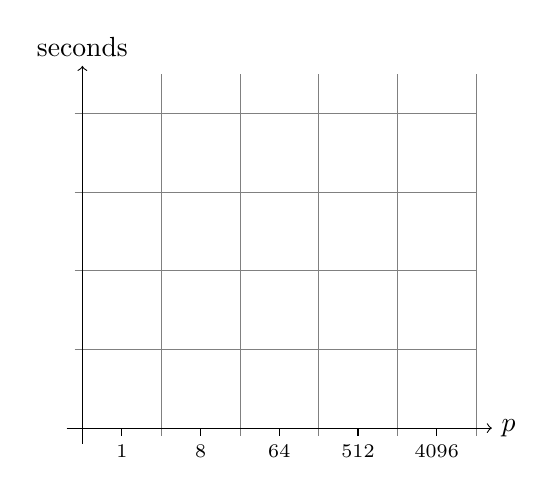
\begin{tikzpicture}[scale=1.0]

\draw[very thin, color=gray] (-0.1,-0.1) grid (5, 4.5);
\draw[->] (-0.2, 0) -- (5.2, 0) node[right] {$p$};
\draw[->] (0, -0.2) -- (0, 4.6) node[above] {seconds};

\foreach \pos/\label in {0.5/1, 1.5/8, 2.5/64, 3.5/512, 4.5/4096}
\draw (\pos,0) -- (\pos,-0.1) (\pos cm,-2.5ex) node [anchor=base,fill=white,inner sep=1pt]  {\scriptsize \label};

%\draw[very thin,color=gray, xstep=1, ystep=0.5] (0, -4.5) grid (13,-0.5);
%\draw[fill=blue!50, fill opacity=0.5] (-3,-1.0) rectangle +(3,0.5);
%\draw (-1.5, -0.75) node {\scriptsize Octree Construction};
%
%\draw[fill=red!50, fill opacity=0.5] (-3,-1.5) rectangle +(3,0.5);
%\draw (-1.5, -1.25) node {\scriptsize Octree Balancing};
%
%\draw[fill=green!50, fill opacity=0.5] (-3,-2.0) rectangle +(3,0.5);
%\draw (-1.5, -1.75) node {\scriptsize Meshing };
%
%\draw[fill=orange!50, fill opacity=0.5] (-3,-2.5) rectangle +(3,0.5);
%\draw (-1.5, -2.25) node {\scriptsize \texttt{MatVec} (5)};
%
%\draw (-3,-3.0) rectangle +(3,0.5);
%\draw (-1.5, -2.75) node {\scriptsize Points};
%
%\draw (-3,-3.5) rectangle +(3,0.5);
%\draw (-1.5, -3.25) node {\scriptsize Unbalanced Octants};
%
%\draw (-3,-4.0) rectangle +(3,0.5);
%\draw (-1.5, -3.75) node {\scriptsize Balanced Octants};
%
%\draw (-3,-4.5) rectangle +(3,0.5);
%\draw (-1.5, -4.25) node {\scriptsize Independent Vertices};
%
%\draw (-2.5ex, 0 cm) node [anchor=base,fill=white,inner sep=1pt] {\scriptsize 0};
%
%\draw (-2.5ex, 1 cm) node [anchor=base,fill=white,inner sep=1pt] {\scriptsize 25};
%
%\draw (-2.5ex, 2 cm) node [anchor=base,fill=white,inner sep=1pt] {\scriptsize 50};
%
%\draw (-2.5ex, 3 cm) node [anchor=base,fill=white,inner sep=1pt] {\scriptsize 75};
%
%\draw (-2.5ex, 4 cm) node [anchor=base,fill=white,inner sep=1pt] {\scriptsize 100};
%
%\newdimen\mypos
%\newdimen\myoff
%
%\foreach \pos/\vala/\valb/\valc/\vald in { 0/0.99/5.34/16.01/18.61, 1/1.41/8.39/23.57/20.72, 2/1.32/8.75/23.19/21.09, 3/1.40/10.55/25.15/20.59, 4/1.44/11.94/26.77/23.29, 5/1.60/12.57/28.99/27.79, 6/1.51/13.52/27.03/25.78, 7/1.65/13.62/29.52/27.65, 8/1.72/14.67/34.91/33.01, 9/1.75/15.99/35.56/31.12, 10/2.17/18.53/36.63/32.40, 11/2.92/25.42/38.23/33.24, 12/6.68/34.44/41.14/28.27} { 
%\mypos=\pos cm
%\advance \mypos by 0.5 cm
%\draw (\mypos, -0.75 cm) node {\scriptsize \vala};
%\draw (\mypos, -1.25 cm) node {\scriptsize \valb};
%\draw (\mypos, -1.75 cm) node {\scriptsize \valc};
%\draw (\mypos, -2.25 cm) node {\scriptsize \vald};
%
%\myoff=0 cm
%
%\advance \mypos by -0.25 cm
%\draw[fill=blue!50, fill opacity=0.5, yscale=0.03980718485307666] (\mypos,\myoff) rectangle +(0.5,\vala);
%\advance \myoff by \vala cm
%\draw[fill=red!50, fill opacity=0.5, yscale=0.03980718485307666] (\mypos,\myoff) rectangle +(0.5,\valb);
%\advance \myoff by \valb cm
%\draw[fill=green!50, fill opacity=0.5, yscale=0.03980718485307666] (\mypos,\myoff) rectangle +(0.5,\valc);
%\advance \myoff by \valc cm
%\draw[fill=orange!50, fill opacity=0.5, yscale=0.03980718485307666] (\mypos,\myoff) rectangle +(0.5,\vald);
%\advance \myoff by \vald cm
%
%}
%
%\draw (0.5, -2.75) node {\scriptsize 180K};
%\draw (0.5, -3.25) node {\scriptsize 607K};
%\draw (0.5, -3.75) node {\scriptsize 996K};
%\draw (0.5, -4.25) node {\scriptsize 660K};
%\draw (1.5, -2.75) node {\scriptsize 361K};
%\draw (1.5, -3.25) node {\scriptsize 1.2M};
%\draw (1.5, -3.75) node {\scriptsize 2M};
%\draw (1.5, -4.25) node {\scriptsize 1.3M};
%\draw (2.5, -2.75) node {\scriptsize 720K};
%\draw (2.5, -3.25) node {\scriptsize 2.4M};
%\draw (2.5, -3.75) node {\scriptsize 4M};
%\draw (2.5, -4.25) node {\scriptsize 2.7M};
%\draw (3.5, -2.75) node {\scriptsize 1.47M};
%\draw (3.5, -3.25) node {\scriptsize 4.9M};
%\draw (3.5, -3.75) node {\scriptsize 8M};
%\draw (3.5, -4.25) node {\scriptsize 5.2M};
%\draw (4.5, -2.75) node {\scriptsize 2.89M};
%\draw (4.5, -3.25) node {\scriptsize 9.7M};
%\draw (4.5, -3.75) node {\scriptsize 16M};
%\draw (4.5, -4.25) node {\scriptsize 10.5M};
%\draw (5.5, -2.75) node {\scriptsize 5.8M};
%\draw (5.5, -3.25) node {\scriptsize 19.6M};
%\draw (5.5, -3.75) node {\scriptsize 31.9M};
%\draw (5.5, -4.25) node {\scriptsize 21.5M};
%\draw (6.5, -2.75) node {\scriptsize 11.7M};
%\draw (6.5, -3.25) node {\scriptsize 39.3M};
%\draw (6.5, -3.75) node {\scriptsize 64.4M};
%\draw (6.5, -4.25) node {\scriptsize 42M};
%\draw (7.5, -2.75) node {\scriptsize 23.5M};
%\draw (7.5, -3.25) node {\scriptsize 79.3M};
%\draw (7.5, -3.75) node {\scriptsize 131M};
%\draw (7.5, -4.25) node {\scriptsize 87.8M};
%\draw (8.5, -2.75) node {\scriptsize 47M};
%\draw (8.5, -3.25) node {\scriptsize 158M};
%\draw (8.5, -3.75) node {\scriptsize 257M};
%\draw (8.5, -4.25) node {\scriptsize 172M};
%\draw (9.5, -2.75) node {\scriptsize 94M};
%\draw (9.5, -3.25) node {\scriptsize 315M};
%\draw (9.5, -3.75) node {\scriptsize 519M};
%\draw (9.5, -4.25) node {\scriptsize 339M};
%\draw (10.5, -2.75) node {\scriptsize 188M};
%\draw (10.5, -3.25) node {\scriptsize 635M};
%\draw (10.5, -3.75) node {\scriptsize 1.04B};
%\draw (10.5, -4.25) node {\scriptsize 702M};
%\draw (11.5, -2.75) node {\scriptsize 376M};
%\draw (11.5, -3.25) node {\scriptsize 1.26B};
%\draw (11.5, -3.75) node {\scriptsize 2.05B};
%\draw (11.5, -4.25) node {\scriptsize 1.36B};
%\draw (12.5, -2.75) node {\scriptsize 752M};
%\draw (12.5, -3.25) node {\scriptsize 2.52B};
%\draw (12.5, -3.75) node {\scriptsize 4.16B};
%\draw (12.5, -4.25) node {\scriptsize 2.72B};

\end{tikzpicture}


	\end{center}
\caption{\label{f:isoUniform} Isogranular scalability for an uniform point distribution.} 
\end{figure}


%\section{Conclusions} \label{sc:conclusions}
%\input{conclusions.tex}

\newpage

%\appendix
%\input{appendix.tex}	

\bibliography{fgt}
\bibliographystyle{plain}
\end{document}


